\chapter{Ferramenta de Apoio de Protocolos de Experimentação}
\label{cp:prototipo}

Neste capítulo são apresentados detalhes da estrutura, arquitetura e implementação da ferramenta de modelagem de modelos de processo de negócio para a concepção de protocolos de experimentação, e a adição destes em pacotes de laboratórios instanciados pela \textit{OntoExpTool}~\cite{Pucci2014}.

A ferramenta tem como propósito oferecer os elementos necessários para a construção de modelos de processo que representem o conjunto de atividades executadas durante o processo experimental por meio da construção de um protocolo de experimentação e a vinculação dos produtos oriundos da experimentação às suas respectivas atividades.

\section{Estrutura da Ferramenta}

Na Figura~\ref{img:workflow} apresenta da sequência de atividades para este trabalho. Essa consiste em um conjunto de atividades que buscam representar através de modelos de processo de negócio cada fase do processo de experimentação em experimentos controlados, ou seja, todas as tarefas relativas às fases de \textit{Definição}, \textit{Planejamento}, \textit{Operação}, \textit{Análise e Interpretação}, e por último, o \textit{Empacotamento}.

%figura
\begin{figure}[!htb]
\centering
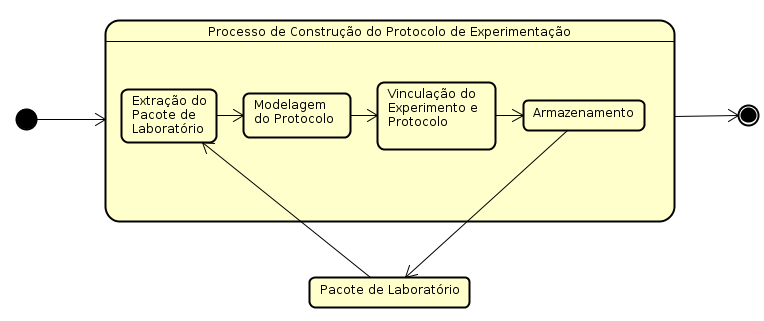
\includegraphics[width=\textwidth]{images/workflow.png}
\caption{Sequência de atividades para a concepção e construção de protocolos de experimentação.}
\label{img:workflow}
\end{figure}


A partir desse processo, foi elaborado o Diagrama de Casos de Uso, ilustrado na Figura~\ref{img:casosdeuso}, tanto no papel de experimentador, para a concepção e construção do protocolo de experimentação, quanto no papel de replicador, para a visualização do protocolo.


%figura
\begin{figure}[!htb]
\centering
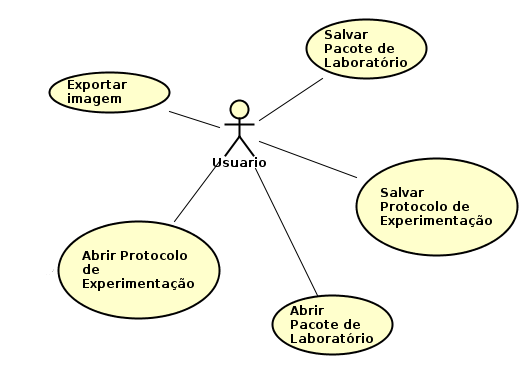
\includegraphics[width=0.7\textwidth]{images/casosdeuso.png}
\caption{Diagrama de Casos de Uso.}
\label{img:casosdeuso}
\end{figure}


Para cada atividade no Diagrama de Casos de Uso, foi gerado um Diagrama de Sequência, os quais são apresentados na Seção~\ref{sect:sequencia}.


\section{Arquitetura da Ferramenta}

A ferramenta foi desenvolvida segundo a arquitetura de camadas~\textit{MVC (Model--View--Controller)}.
A primeira camada -- \textit{View} -- corresponde ao conjunto de elementos \textit{JavaServer Pages} (JSPs), responsáveis  pela interação do usuário com o sistema. Neste sistema, são providos os elementos necessários para a construção dos modelos de processo de negócio. Os JSPs trocam mensagens com os \textit{Servlets}.

A segunda camada -- \textit{Controller} -- é composta pelos \textit{Servlets} e controladores, sendo responsáveis pelo tratamento dos dados enviados pela camada anterior, assim como realizar a interação com o \textit{Model}. A troca de dados é realizada por meio do método POST do protocolo HTTP (\textit{Hypertext Transfer Protocol}) utilizando a tecnologia AJAX (\textit{Asynchronous JavaScript and XML}) com a notação de objeto de dados JSON (\textit{JavaScript Object Notation}).

Por fim, a terceira camada -- \textit{Model} -- é responsável pela manipulação e validação modelo do sistema, correspondendo ao processo de negócio da ferramenta. Esta camada faz a interação com a persistência de dados, que usa um modelo de banco de dados não-relacional orientado a documentos, tendo \textit{XML} como linguagem -- ressalta-se que o próprio modelo deve ser persistido.

\section{Diagramas de Sequência}
\label{sect:sequencia}


\subsection{Caso de Uso - Abrir Protocolo}

Para a primeira atividade de Caso de Uso foi elaborado o seguinte Diagrama de Sequência -- Abrir Protocolo -- apresentado na Figura~\ref{img:abrirprotocolo}, no qual o usuário extrai somente o protocolo de experimentação, seja apenas para a visualização de seu conteúdo ou também para sua manipulação e aplicação de alterações sob o protocolo.

%figura
\begin{figure}[!htb]
\centering
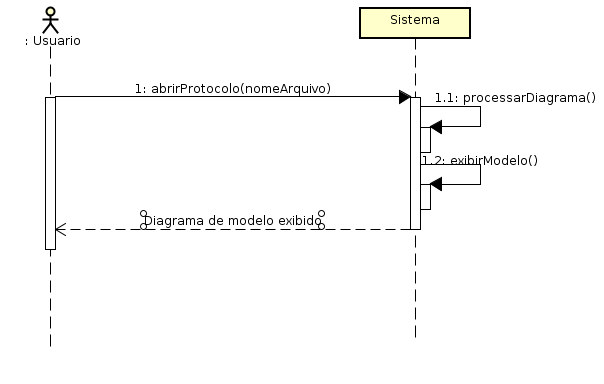
\includegraphics[width=0.8\textwidth]{images/abrirprotocolo.png}
\caption{Diagrama de Sequência -- Abrir Protocolo.}
\label{img:abrirprotocolo}
\end{figure}


\subsection{Caso de Uso - Salvar Protocolo}

Para este Caso de Uso, foi elaborado o Diagrama de Sequência -- Salvar Protocolo -- representado na Figura~\ref{img:salvarprotocolo} no qual, sob o papel de experimentador, o usuário da ferramenta após a construção parcial ou total do modelo de processo de negócio solicita o armazenamento do diagrama na forma de um diagrama BPMN e, em seguida, fornece o nome do arquivo para o processo de gravação.

%figura
\begin{figure}[!htb]
\centering
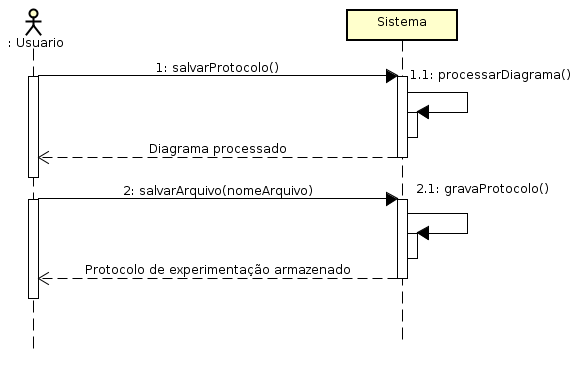
\includegraphics[width=0.8\textwidth]{images/salvarprotocolo.png}
\caption{Diagrama de Sequência -- Salvar Protocolo.}
\label{img:salvarprotocolo}
\end{figure}


\subsection{Caso de Uso - Abrir Pacote}

Para este Caso de Uso, foi criado o Diagrama de Sequência -- Abrir Pacote -- o qual está ilustrado na Figura~\ref{img:abrirpacote}, no qual, tanto no papel de experimentador quanto replicador, o usuário a partir de um arquivo fornecido (Pacote de Laboratório) tem acesso de visualização e manipulação do protocolo de experimentação, assim como a consulta de informações textuais do experimento e do relacionamento entre itens do experimento com suas respectivas atividades no protocolo.

%figura
\begin{figure}[!htb]
\centering
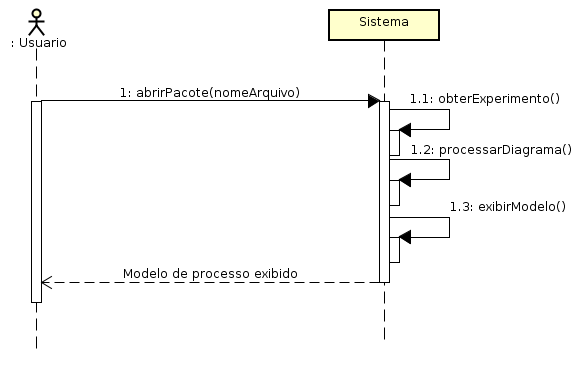
\includegraphics[width=0.8\textwidth]{images/abrirpacote.png}
\caption{Diagrama de Sequência -- Abrir Pacote.}
\label{img:abrirpacote}
\end{figure}


\subsection{Caso de Uso - Salvar Pacote}

A partir deste Caso de Uso, foi elaborado o Diagrama de Sequência -- Salvar Pacote -- apresentado pela Figura~\ref{img:salvarpacote}, o usuário, no papel de experimentador, manipula o conteúdo referente ao modelo de processo de negócio e, em seguida, solicita o armazenamento das alterações fornecendo o nome do arquivo para gravação. Como restrição, este pacote de laboratório deve ter sido instanciado previamente contendo informações do experimento.

%figura
\begin{figure}[!htb]
\centering
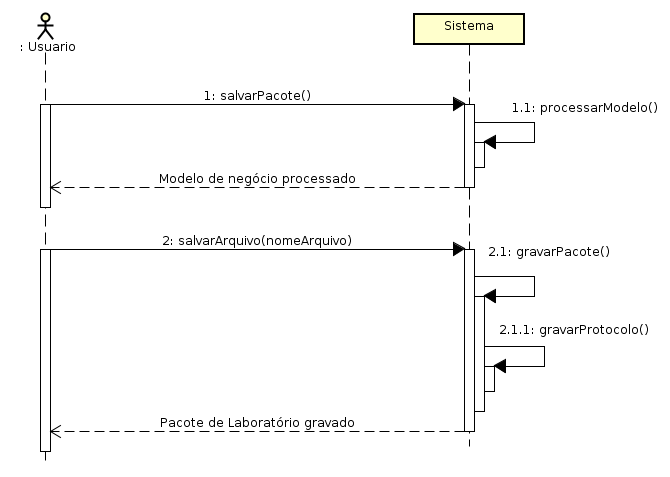
\includegraphics[width=0.8\textwidth]{images/salvarpacote.png}
\caption{Diagrama de Sequência -- Salvar Pacote.}
\label{img:salvarpacote}
\end{figure}


\subsection{Caso de Uso - Exportar Imagem}

Por fim, neste último Caso de Uso, foi elaborado o Diagrama de Sequência -- Exportar Imagem -- representado na Figura~\ref{img:exportarimagem}, no qual, a partir de um modelo de processo construído manualmente, extraído de um protocolo ou pacote de laboratório é possível obter uma versão deste no formato de imagem, através da solicitação desta função e fornecimento do nome do arquivo para a gravação.

%figura
\begin{figure}[!htb]
\centering
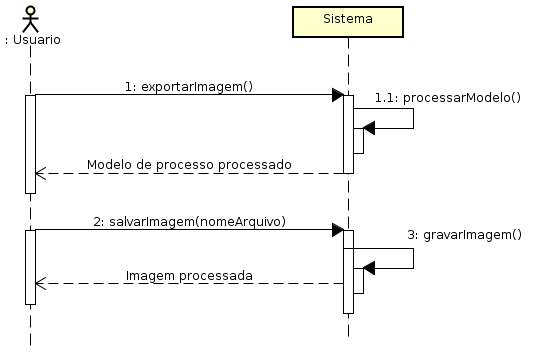
\includegraphics[width=0.8\textwidth]{images/exportarimagem.png}
\caption{Diagrama de Sequência -- Exportar Imagem.}
\label{img:exportarimagem}
\end{figure}


\section{Diagramas de Classes}

Foram elaborados dois Diagramas de Classes; em que no primeiro (Figura~\ref{img:classesexperimento}), é apresentada a camada de persistência relativa ao experimento; enquanto o segundo, ilustrado na Figura~\ref{img:classesmodelo}, contém a camada de persistência relativa ao modelo de processo de negócio utilizado para a construção do protocolo de experimentação.


%figura
\begin{figure}[!htb]
\centering
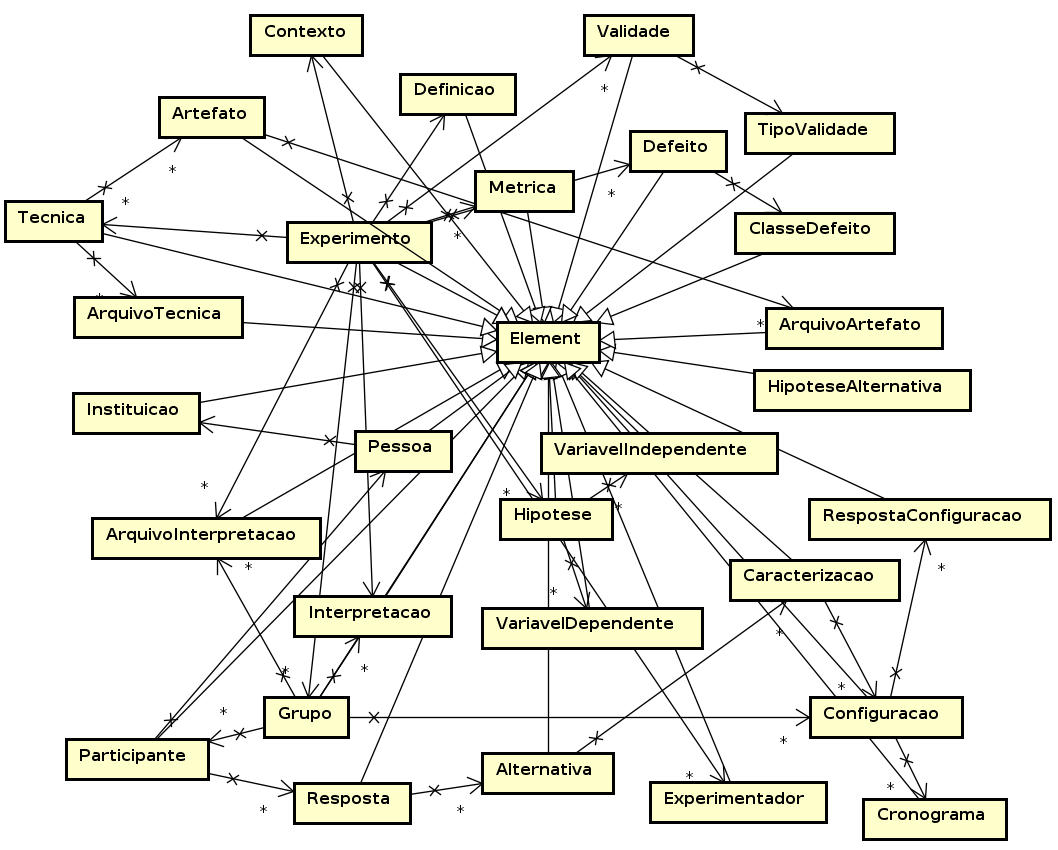
\includegraphics[width=\textwidth]{images/classesexperimento.png}
\caption{Diagrama de Classes do Experimento -- Simplificado.}
\label{img:classesexperimento}
\end{figure}

\begin{landscape}

%figura
\begin{figure}[!htb]
\centering
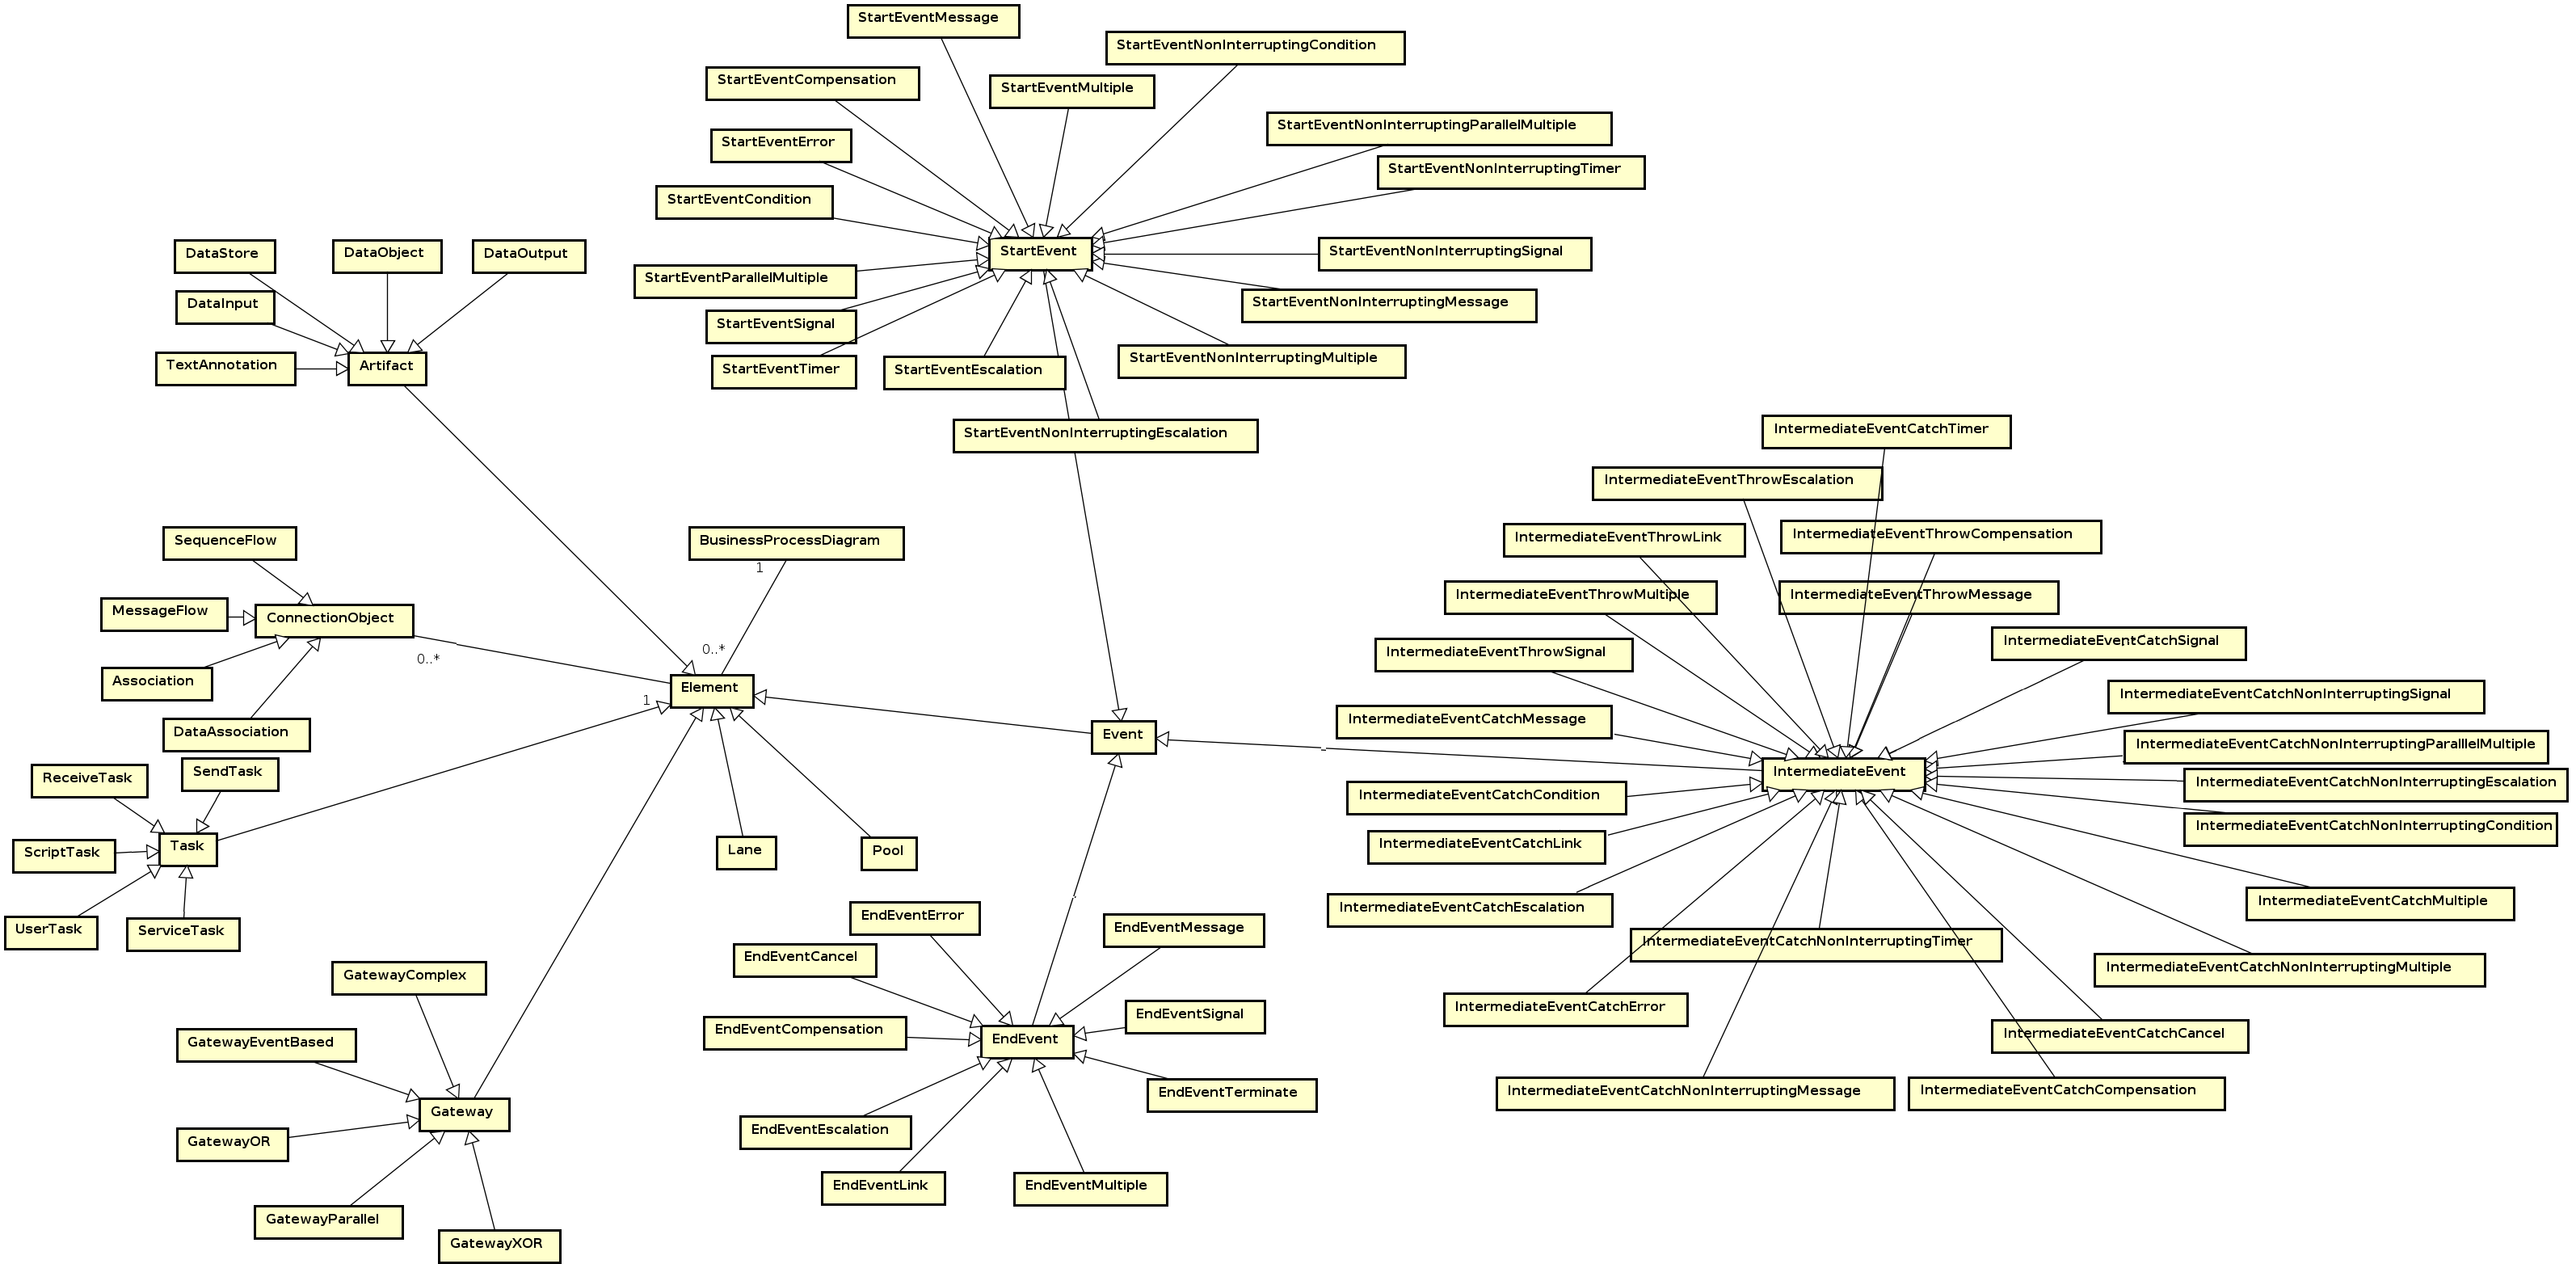
\includegraphics[width=1.55\textwidth]{images/classesbpmn.png}
\caption{Diagrama de Classes do Modelo de Processo -- Simplificado.}
\label{img:classesmodelo}
\end{figure}

\end{landscape}

\section{Implementação da Ferramenta}

A ferramenta foi implementada utilizando a linguagem de programação de Java, com foco em aplicações web, servidor GlassFish Server 4.1 e o ambiente de desenvolvimento integrado NetBeans 8.2. A aplicação tem como plataforma o ambiente \textit{web}, logo independente de sistema operacional.

Adicionalmente, foram utilizadas algumas bibliotecas e tecnologias auxiliares para prover maior estabilidade à aplicação e atender os objetivos planejados, tais como:

\begin{itemize}
\item \textit{jQuery}: biblioteca JavaScript utilizada para simplificar o desenvolvimento
e codificação de HTML, facilitando a manipulação do conjunto de elemento do DOM HTML, assim como a adição de efeitos visuais e uma interface para requisições AJAX mais simples e intuitiva.

\item \textit{AJAX}: tecnologia responsável pela realização de requisições e troca de informações entre o navegador (cliente) e o servidor \textit{web} sem a necessidade do recarregamento total da página HTML, de modo a prover uma melhor experiência do usuário com a ferramenta.

\item \textit{XStream}: é uma biblioteca Java utilizada na serialização e desserealização de objetos para o formato XML e JSON. Utilizada nos processos de leitura e gravação dos arquivos referentes ao protocolo de experimentação e ao pacote de laboratório.

\item \textit{D3.js}: consiste em uma biblioteca JavaScript para manipulação de elementos HTML, com foco principal em elementos gráficos e manipulação de elementos SVG, que neste projeto se referem aos itens da notação BPM. 

\end{itemize}

Em relação à persistência de dados na ferramenta, todos os dados são armazenados seguindo o modelo de dados não-relacional orientado a documentos, utilizando a linguagem de marcação XML, tanto para os protocolos de experimentação quanto para o pacote de laboratório.

Na Listagem~\ref{ls:pacote-xml} apresenta um trecho do código referente à descrição de um pacote de laboratório.

\lstset{language=XML}
\begin{lstlisting}[caption=Descrição reduzida de um pacote de laboratório., label=ls:pacote-xml]
<Experimento>
  <id>experimento0</id>
  <status>0</status>
  <replicacao>0</replicacao>
  <diagrama>
    <elements>
      <Pool>
        <id>#pool0</id>
        <x>451</x>
        <y>221</y>
        <description>Exemplo</description>
        <name>participant</name>
        <type>BPMNLane</type>
        <elements>
          <Lane>
           ...
          </Lane>
        </elements>
        <transitions/>
        <width>600</width>
      </Pool>
    </elements>
  </diagrama>
  <experimentadores/>
  <definicao>
    <id>definicao1</id>
    <protegido>false</protegido>
  </definicao>
  <contexto>
    <id>contexto2</id>
    <protegido>false</protegido>
  </contexto>
  <hipoteses/>
  <validades/>
  <metricas/>
  <tecnicas/>
  <defeitos/>
  <grupos/>
  <interpretacao/>
  <arquivoInterpretacao/>
</Experimento>

\end{lstlisting}

\section{Interface da Ferramenta}
A ferramenta de construção de protocolos de experimentação foi desenvolvida visando uma simples manipulação dos itens para a elaboração dos respectivos diagramas. A Figura~\ref{img:janela} representa um instantâneo da aplicação durante a processo de um modelo de processo de negócio.

\begin{figure}[!htb]
\centering
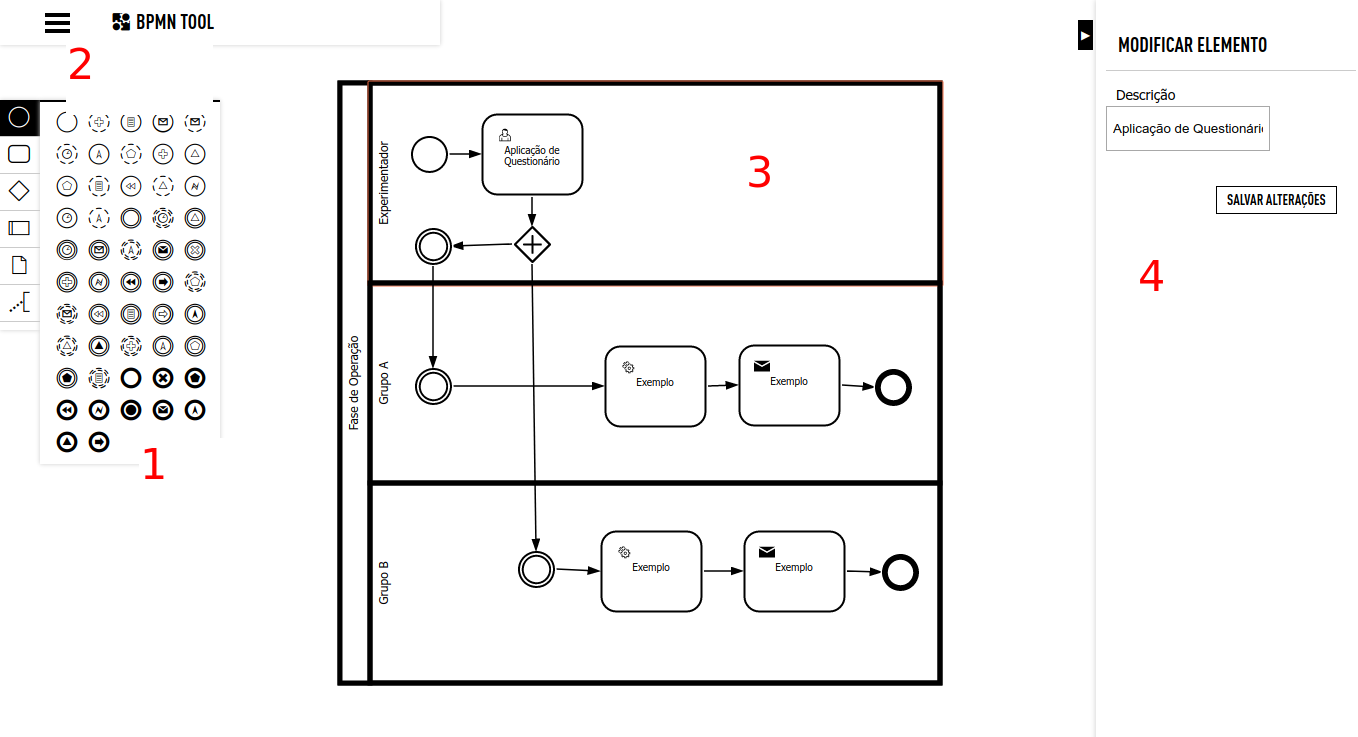
\includegraphics[width=\textwidth]{images/janelaferramenta.png}
\caption{Instantâneo da ferramenta de construção de protocolo de experimentação.}
\label{img:janela}
\end{figure}

A interface de interação com usuário foi subdividida em quatro áreas, como indicado na Figura~\ref{img:janela}, cujos propósitos foram descritos a seguir:

\begin{itemize}
\item Área 1 -- \textit{Seleção de Elementos} -- nesta área da aplicação, o usuário tem acesso aos elementos gráficos que compõem a notação BPMN, permitindo a seleção e, consequentemente adição ao protocolo de experimentação.

\item Área 2 -- \textit{Lista de Menus} -- nesta parte da aplicação estão presentes os menus que permitem a leitura e gravação de protocolos de experimentação e pacotes de laboratório, assim como, a exportação no formato imagem.

\item Área 3 -- \textit{Área de Modelagem} -- esta área da aplicação é destinada a modelagem dos diagramas de processo de negócio, através da manipulação dos elementos pertinentes à notação, construindo a transição, raias e piscinas.

\item Área 4 -- \textit{Painel de Detalhes} -- este painel viabiliza a alteração de atributos dos elementos pertencentes a modelagem, permitindo a modificação de atributos como largura e altura, e texto de descrição, por exemplo.
\end{itemize}




\section{Considerações Finais}
Neste capítulo foram apresentados os detalhes referentes estrutura, arquitetura e implementação da ferramenta de modelagem de modelos de processo de negócio, que viabiliza a construção de protocolos de experimentação (plano de execução), e a  respectiva adição em pacotes de laboratórios instanciados pela \textit{OntoExpTool} baseados na ontologia \textit{ExperOntology}.

No próximo capítulo é apresentado o processo de construção de protocolo de experimentação referente ao estudo de trabalho executado no trabalho de~\citeauthoronline{d2012avaliaccao}~(\citeyear{d2012avaliaccao}).
